%% article.tex -- IEEE/IFIP NOMS submission (full technical paper)
%%
%% Session-Centric Knowledge Graphs for Explainable Detection and
%% Scoped Mitigation of Application-Layer DDoS
%%
%% Target: IEEE/IFIP NOMS 2027 (technical session, full paper).
%% Format: IEEEtran conference, 2 columns, 10pt, US letter.
%% Rules taken from the NOMS 2026 CFP (re-verify when the 2027 CFP is out):
%%   - up to 8 pages of MAIN TEXT, self-contained;
%%   - references and an optional appendix may add pages, 12 total maximum;
%%   - single-blind review, so authors are named;
%%   - over-length papers are rejected without review.
%% Current layout: main text pp.1-7, references p.7-8, appendices pp.8-9.

\documentclass[conference,letterpaper,10pt]{IEEEtran}
\IEEEoverridecommandlockouts

\usepackage[T1]{fontenc}
\usepackage[utf8]{inputenc}
\usepackage{cite}
\usepackage{amsmath,amssymb}
\usepackage{graphicx}
\usepackage{booktabs}
\usepackage{algorithm}
\usepackage{algorithmic}
\usepackage{url}
\usepackage[hidelinks]{hyperref}

%% IEEEtran uses URW Courier (pcr) for \texttt. Fall back to Computer Modern
%% typewriter when those metrics are absent locally; Overleaf and full TeX Live
%% installations keep the IEEE-standard font.
\IfFileExists{pcrr8t.tfm}{}{\renewcommand{\ttdefault}{cmtt}}

\def\BibTeX{{\rm B\kern-.05em{\sc i\kern-.025em b}\kern-.08em T\kern-.1667em\lower.7ex\hbox{E}\kern-.125emX}}

\begin{document}

\title{Session-Centric Knowledge Graphs for Explainable\\Detection and Scoped Mitigation of Application-Layer DDoS}

\author{\IEEEauthorblockN{Natanael Oliveira, Arthur Kobielski, and Marcos Luna}
\IEEEauthorblockA{Institute of Informatics, Universidade Federal do Rio Grande do Sul (UFRGS), Porto Alegre, Brazil\\
\{natanael.oliveira, arthur.kobielski, marcos.luna\}@inf.ufrgs.br}}

\maketitle

\begin{abstract}
Distributed Slow HTTP DoS campaigns keep every source below any reasonable
per-session threshold, so the attack signal lives in the structure \emph{between}
sessions rather than inside any one of them --- and detectors discard that
structure by reducing the session to a numeric vector, while recent
knowledge-graph detectors reason at the network-node level and stop at a textual
report. We model the HTTP session as a first-class ontological entity in OWL and
replace the flat \texttt{relatedTo} link with six typed sub-properties weighted
by the attacker's cost of breaking each signal, network proximity ranking lowest
because modern botnets distribute aggressively across ASNs and prefixes. A
SPARQL/SWRL rule fires on their weighted mass, and its derivation \emph{is} the
verdict, exported as a JSON-LD and STIX~2.1 evidence chain whose discriminator
scopes the mitigation. Against stealthy distributed campaigns, per-session
detection stays at chance across four model families given the full flow-feature
set, while cross-session reasoning detects them consistently (ROC AUC $0.50$
vs.\ $0.98$; $d = 22.4$); on public datasets, whose attacks carry an obvious flow
signature, a strong per-session baseline already suffices --- a boundary we report
explicitly. We further show that the obvious way to scope the mitigation is
harmful: the property most of the cluster shares is a \emph{legitimate}
fingerprint once the botnet spans several TLS stacks, blocking $0\%$ of the attack
and $39\%$ of the users. Choosing the discriminator by enrichment over a profile
of normal traffic blocks $85$--$90\%$ at $0.00\%$ collateral instead, and as a
detector that symbolic path needs no training or threshold, recovering two to five
times more of a fragmented campaign than the learned model can at the same
zero-false-positive operating point.
\end{abstract}

\begin{IEEEkeywords}
security management, knowledge graph, application-layer DDoS, semantic models,
automated reasoning, explainability, mitigation policy
\end{IEEEkeywords}

%% ====================================================================
\section{Introduction}
\label{sec:intro}

Application-layer DDoS has changed in kind, not only in scale. In August 2023,
HTTP/2 Rapid Reset (CVE-2023-44487) pushed mitigated peaks to 398 million
requests per second from a botnet of roughly twenty thousand
machines~\cite{cve202344487,google2023rapidreset}, and Cloudflare blocked more
than 6\,500 hyper-volumetric attacks in Q2 2025 alone, with HTTP DDoS growing
129\% year over year~\cite{cloudflare2025q2ddos}. Volumetric defences answer the
loud end of this spectrum. The quiet end is harder. The family of
\emph{distributed Slow HTTP DoS} attacks covers Slowloris and its descendants,
plus rate-based variants that still hold connections open, such as HULK and
GoldenEye~\cite{cambiaso2013slowdos}. These exhaust a server from many
coordinated origins, each contributing so little that no per-source threshold is
crossed. Modern HTTP/2 attacks share that multi-origin exhaustion property, but
they operate through distinct mechanisms, notably stream cancellation and header
continuation abuse. Those call for sub-relations outside the scope we evaluate
here, and we treat them as the immediate extension target
(Section~\ref{sec:conclusion}) rather than as a claim of this paper.

Seen in isolation, every request is indistinguishable from a legitimate one. The
signal lives in the structure \emph{between} sessions: connection duration,
route entropy, client fingerprint consistency, and the convergence of many
origins on one endpoint under one client signature~\cite{kemp2023approach}.

This is a network and service management problem as much as a detection problem.
An operator does not need a label; the operator needs to know \emph{which}
clients to act on, on \emph{what} evidence, and with a filter narrow enough not
to disconnect the legitimate users of the very service under attack.

The literature acknowledges the first half and largely ignores the second. The
meta-analysis of Odusami et al.~\cite{odusami2020survey} over seventy-five
studies finds that 47\% of application-layer DDoS methods derive features from
sessions, such as request rate per user, mean duration and operations per
identity. In all of them the session is flattened into a numeric vector before it
reaches the classifier. The detector sees statistics, not sessions, and
therefore cannot reason about reused identities, about fingerprints converging
on an endpoint, or about patterns that only exist between two individually
normal sessions.

Contemporary work attacks the opacity of these detectors with graphs. KLAGE, by
Belcastro et al.~\cite{belcastro2025klage}, builds knowledge graphs from network
logs, classifies nodes with Graph-BERT, and produces natural-language reports
via LIME and large language models, reaching $F_1 = 84.1\%$ on IoT benchmarks
that include DDoS Slowloris. It is solid evidence that knowledge graphs are a
viable runtime detection substrate. Three properties, however, remain open. Its reasoning unit is the \emph{network
node} (port, IP, flow) rather than the application session. Coordination is
captured implicitly in learned embeddings rather than in named symbolic relations.
And the pipeline ends at a report, without a mitigation policy whose scope is
derived from the graph itself. Those
three gaps define the space this paper occupies.

\textbf{Contributions.} We make four:

\begin{enumerate}
\item \textbf{The HTTP session as a first-class ontological entity, with a
weighted \texttt{relatedTo} family.} An OWL ontology models
\texttt{ApplicationSession} with typed relations to client identity, target
endpoint, exhibited behavior and applicable mitigation, and replaces the flat
\texttt{relatedTo} link with a family of \emph{six typed, weighted}
sub-properties. The weights encode the attacker's cost of breaking each signal. Network
proximity, trivially broken by modern botnets, therefore enters as auxiliary
evidence and never as a prerequisite.

\item \textbf{Symbolic reasoning over a weighted sum of sub-relations.} A
runtime pipeline lifts HTTP events into ontology instances, instantiating each
sub-property independently from its own evidence. A SPARQL/SWRL rule fires on the
weighted coordination mass $\Omega(S)$ of a candidate cluster. The verdict is the
derivation that satisfied the rule, not a classifier output interpreted after the
fact.

\item \textbf{An evidence chain coupled to automatic mitigation scoping.} Each
verdict carries a JSON-LD and STIX~2.1 chain listing the activated
sub-relations, their weights and the values that satisfied the rule, and the scope
of the mitigation is derived from the same graph. We show that the natural way to
derive it --- the property most of the cluster shares --- is actively harmful under
realistic conditions, and replace it with a criterion based on enrichment over a
profile of normal traffic.

\item \textbf{An evaluation parameterised by the degree of distribution, with a
collateral-damage metric.} Against a deliberately \emph{strong} per-session baseline, ablation isolates the
gain of cross-session reasoning and the specific gain of high-weight signals over
network proximity. We also report the fraction of legitimate traffic hit by the
resulting mitigation, a metric self-reported by commercial bot-management products
but, to our knowledge, not used systematically in the academic Layer-7
literature. The reference implementation
is open source.
\end{enumerate}

Section~\ref{sec:related} positions the work, Section~\ref{sec:approach}
presents the framework, Sections~\ref{sec:method} and~\ref{sec:results} the
methodology and results, and Section~\ref{sec:discussion} the limitations that
bound the claim.

%% ====================================================================
\section{Related Work}
\label{sec:related}

\subsection{Knowledge Graphs for Security and Management}

The first wave of security knowledge graphs was \emph{static}: entities
extracted from CVEs, reports and blogs, normalised and linked into a queryable
base~\cite{jia2018practical,bonagiri2024practical}. The survey of Liu et
al.~\cite{liu2022recent} states the resulting gap plainly: ``it is still
unclear how to implement the knowledge graph to face real industrial
difficulties in cyber attack and defense situations''. Graphs built from threat
intelligence text do not capture runtime traffic structure.

More recent work populates graphs from traffic itself. KLAGE~\cite{belcastro2025klage}
is the closest exemplar and the one we compare against. Graph representations
are also gaining ground in management tasks adjacent to ours: Sadlek et
al.~\cite{sadlek2024device} identify device dependencies through link prediction
over network graphs, and Wang and Stadler~\cite{wang2024intrusion} learn attack
action sequences from testbed measurements. Both operate on network-level
entities. We differ from them on three axes. Our reasoning unit is the
application session; our formalism is named symbolic relations rather than
learned embeddings; and our output includes the scope of the mitigation.

\subsection{Layer-7 HTTP DDoS Detection}

Detection organises historically into three families. Statistical profiling
builds baselines from aggregated flow or session statistics: Fernandes et
al.~\cite{fernandes2015autonomous} with PCA over flow statistics, Bharathi and
Sukanesh~\cite{bharathi2012pca} with PCA over a per-session behavioural matrix
which is one of the first formulations to put the session at the centre, though
still as a feature vector. Supervised learning over session features is the second
family, with Kemp et al.~\cite{kemp2023approach} as the most recent
representative; its authors note that the method was not validated in real time
and that the output is binary, without ontological explanation. The third family
consolidates the domain in surveys~\cite{tripathi2021application,cambiaso2013slowdos}.
The common denominator is that the session is treated as a feature aggregate,
never as an entity one can reason about.


\subsection{Session Modelling in Anomaly Detection}

The meta-analysis of Odusami et al.~\cite{odusami2020survey} gives the clearest
quantitative evidence of how the session is handled: in 47\% of the catalogued
methods, session-derived features feed the classifier, yet in none of the
seventy-five studies is the session kept as an object with identity, target,
behavior and typed relations. The reduction is uniform, and it is what puts
reasoning about reused identities, about fingerprints converging on an endpoint,
or about patterns visible only across sessions out of the detector's reach.

Industrial bot-management platforms do exploit cross-session structure, grouping
apparently independent sessions by TLS stack similarity through JA4-family
fingerprints~\cite{althouse2023ja4}. They are proprietary, however, with no public
ontology, no reproducible academic benchmark, and no formalised collateral-damage
metric. Formalising that practice auditably, and deriving mitigation scope from
an explicit ontological rule, is what remains open.

%% ====================================================================
\section{Session-Centric Knowledge Graph}
\label{sec:approach}

\begin{figure*}[t]
\centering

\includegraphics[width=0.72\textwidth]{figures/fig1_ontology.png}
\caption{Session-centric ontology. \texttt{ApplicationSession} is a first-class
entity with typed primary relations to identity, origin, endpoint and behavior;
the weighted \texttt{relatedTo} family links sessions to each other; and the
detection rule couples the symbolic verdict to a course of action whose scope is
derived from the coordinated subset.}
\label{fig:ontology}
\end{figure*}

Fig.~\ref{fig:ontology} summarises the framework. Four stages run over live
traffic: HTTP events are ingested; lifted into ontology instances with sessions
as persistent graph nodes; evaluated by semantic rules; and turned into a verdict
carrying its evidence chain and derived mitigation scope.

\subsection{Ontology}
\label{sec:ontology}

The central class is \texttt{ApplicationSession}, related by
\texttt{hasIdentity} to a composite \texttt{Identity} (cookie, JWT token,
username, TLS fingerprint), by \texttt{targets} to an \texttt{Endpoint}
(\texttt{AuthEndpoint}, \texttt{APIEndpoint}, \texttt{StaticAsset}), by
\texttt{exhibitsBehavior} to a behavioural profile, and by \texttt{mitigatedBy}
to a policy (\texttt{RateLimit}, \texttt{Challenge}, \texttt{Block}) carrying a
\texttt{scope} attribute. The abstract class \texttt{ApplicationLayerAttack}
specialises into \texttt{SlowHTTPDoSFamily}, itself split into
\texttt{ConnectionExhaustionAttack} (Slowloris, slow body, slow read) and
\texttt{CoordinatedHTTPFlood} (HULK, GoldenEye). The ontology is aligned with
STIX~2.1~\cite{oasis2021stix} and MITRE ATT\&CK, and also declares
\texttt{CredentialStuffing} and \texttt{CoordinatedAPIAbuse}, which reuse the
same machinery but are outside the experimental scope of this paper.

\subsection{Threat Model}
\label{sec:threat}

The defender operates the attacked application and observes, per request, the TLS
\emph{ClientHello} (hence a JA4 fingerprint), source address and prefix/ASN,
target endpoint, arrival time, and whatever identity material the application
exposes. It does not observe the botnet's control channel and has no ground truth
about which sources are coordinated; it can, however, profile its own traffic
when not under attack. The attacker controls $K$ origins, places them in the
network, and may shape each session to be statistically indistinguishable from a
legitimate one, which is the stealth assumption of our evaluation. It may also break
individual coordination signals: forging JA4 with browser-impersonating
libraries, jittering timing, rotating identities, randomising payloads. Each move
carries an operational cost, and the weighting of Section~\ref{sec:family}
encodes that cost; Sections~\ref{sec:collateral} and~\ref{sec:discussion} report
what happens when the strongest signal is taken away.

\subsection{The Weighted \texttt{relatedTo} Family}
\label{sec:family}


Cross-session relatedness is not one relation but a structured family, declared
via \texttt{rdfs:subPropertyOf} under a transitive \texttt{relatedTo} and
annotated with a \texttt{coordinationWeight} $w_i \in [0,1]$, listed in
Fig.~\ref{fig:ontology}. Each is instantiated independently from its own observed
evidence, so two sessions may be linked by one, several or all six.

The ordering is an evasion-cost argument. Changing the TLS stack forces the
attacker to rewrite infrastructure, which is why JA4 survived the extension
randomisation Chrome introduced in 2023 whereas classic JA3 did
not~\cite{althouse2023ja4}. Identity reuse is equally expensive to break, because
pulverising credentials attacks the economics of the campaign itself. Temporal
coherence emerges from botnet operation rather than from the client stack, and
random jitter can partially break it. Payload and endpoint
signals are middling: randomising them is cheap, but doing so costs campaign
coherence. Network proximity is the weakest link by construction: Mirai
derivatives, cloud fleets and residential-proxy networks spread across ASNs and
prefixes, and carrier-grade NAT makes a shared /24 a poor discriminator. That
weight ordering, not the absolute values, is what the calibration in
Appendix~\ref{app:calibration} corroborates.

\subsection{Runtime Graph Construction}
\label{sec:pipeline}

Sessions and relations live inside a sliding operational window ($W = 5$~min by
default) and are purged incrementally, following an RDF stream-processing
discipline. We adopt the OWL~2~RL profile~\cite{w3c2012owl2profiles}, which
admits forward-chaining materialisation with near-linear behaviour on indexed
SPARQL queries, over Apache Jena Fuseki with TDB2 storage; full OWL~2~DL
reasoners do not scale to graphs of this size. Algorithm~\ref{alg:kg} sketches
construction; the per-pair decision procedure of each \texttt{relatedBy}
sub-relation is given in Appendix~\ref{app:algorithms}. Admitting a new session
into a window holding $|S_W|$ active sessions costs $O(|S_W|\cdot c)$, with $c$
amortised $O(1)$ for every sub-relation except the temporal one, which is
dominated by FastDTW under a Sakoe--Chiba band. Section~\ref{sec:latency}
measures both this admission path and the symbolic layer against window
occupancy.

\begin{algorithm}[t]
\caption{Runtime knowledge-graph construction}
\label{alg:kg}
\begin{algorithmic}[1]
\REQUIRE request stream $\mathcal{R}$, ontology $\mathcal{O}$, window $W$
\ENSURE knowledge graph $KG$ persistent over $W$
\STATE $KG \leftarrow \emptyset$
\FOR{each request $r \in \mathcal{R}$}
  \STATE $s,i,e \leftarrow \textsc{ResolveSession/Identity/Endpoint}(r)$
  \STATE $KG.\mathrm{add}(s,i,e)$; \, $KG.\mathrm{link}(s,\texttt{hasIdentity},i)$
  \STATE $KG.\mathrm{link}(s,\texttt{targets},e)$
  \FOR{each active $s' \in S_W$, $s' \neq s$}
    \FOR{each sub-relation $i \in \mathcal{R}_{\mathrm{rel}}$}
      \IF{$\textsc{Holds}_i(s,s')$}
        \STATE $KG.\mathrm{link}(s,\texttt{relatedBy}_i,s')$
      \ENDIF
    \ENDFOR
  \ENDFOR
  \STATE $KG.\mathrm{purgeOutside}(W)$
\ENDFOR
\RETURN $KG$
\end{algorithmic}
\end{algorithm}

\subsection{Detection Rule}
\label{sec:rule}

Let $V_{\mathrm{sess}}$ be the sessions active in $W$. For a subset $S \subseteq
V_{\mathrm{sess}}$ and a candidate endpoint $e$, define the \emph{coordination
mass}

\begin{equation}
\Omega(S) \;=\; \sum_{i \in \mathcal{R}_{\mathrm{rel}}} w_i \,\big|E_i(S)\big| ,
\label{eq:omega}
\end{equation}

with $E_i(S) = \{\{s_a,s_b\} \subseteq S : (s_a,\texttt{relatedBy}_i,s_b) \in E\}$
the set of session pairs linked by sub-relation $i$. Sub-relations are symmetric,
so each unordered pair counts once. The rule
\texttt{CoordinatedHTTPFlood} is satisfied when there exists $S$ with (i)
$|S| \geq k_{\min}$; (ii) $\forall s \in S: (s,\texttt{targets},e) \in E$; (iii)
$\Omega(S) \geq \tau_{\mathrm{cluster}}$; (iv) aggregate rate on $e$ above
$\tau_{\mathrm{rate}}$; and (v) a coherent \texttt{BotBehavior} profile.

Condition (iii) is the contribution. $\Omega(S)$ can clear the threshold with
\texttt{relatedByNetworkProximity} at zero, which is the distributed-botnet case,
provided some combination of high-weight signals is observed. Conversely, a set
held together \emph{only} by network proximity, such as legitimate mobile users
behind one CGN /24, cannot reach $\tau_{\mathrm{cluster}}$ on $w = 0.3$ alone.
This is explicit protection against a well-known false-positive mode.

\subsection{Symbolic Formulation}
\label{sec:symbolic}

Reasoning is symbolic in two stages, and the split is deliberate.
Pair-wise instantiation of the \texttt{relatedBy} family is pure Horn logic and
is expressed as SWRL rules; aggregation is not, because SWRL cannot sum, so
$\Omega(S)$ is computed by a SPARQL query whose weights are read from the
\texttt{coordinationWeight} annotations in the ontology rather than hard-coded.
Fig.~\ref{fig:rules} shows one rule of each kind.


\subsection{Evidence Chain and Derived Mitigation Scope}
\label{sec:evidence}

When the rule fires, the engine emits the satisfied rule, the ontology instances
involved, the decomposition of $\Omega(S)$ per sub-relation, and the derived
mitigation scope. We export this as JSON-LD over the ontology vocabulary and as
STIX~2.1, an \emph{indicator} plus a \emph{course-of-action} linked by
\emph{mitigates}, for SIEM and SOAR ingestion.

How the scope is chosen decides whether the verdict is useful or harmful, and the
obvious choice is the wrong one. Taking the property shared by \emph{most} of the
cluster, its modal fingerprint, selects whatever is common. On a service under
attack, what is common is the legitimate population. Against a botnet spread over
several TLS stacks, each attacker stack is smaller than the head of the benign
fingerprint distribution, so the modal value is a \emph{legitimate} fingerprint
and the resulting filter blocks users and no attackers. We measure this in
Section~\ref{sec:collateral}.

We therefore select the discriminator by \textbf{enrichment} rather than by
frequency. Let $c(f)$ be the prevalence of fingerprint $f$ inside the fired
cluster and $b(f)$ its prevalence in a background profile of normal traffic
maintained by the operator outside attack episodes. The scope admits every $f$
with $c(f)/b(f) \geq \rho$ and $c(f) \geq \sigma$, yielding a \emph{set} of
fingerprints rather than one, which is what covers a fragmented botnet. The
support floor $\sigma$ must sit below the share of the smallest stack worth acting
on, that is, below $1/M$ for a botnet of $M$ stacks. Lowering it costs nothing,
because it is the enrichment test, not the floor, that keeps legitimate traffic
out. We use $\rho = 3$ and $\sigma = 0.002$.

The background must come from outside the attack episode. Using the window itself
does not work: the campaign spans the whole window, so cluster and background
prevalences coincide and every candidate scores an enrichment of one. No labels
are involved, since the profile is what a defender observes in normal operation.
A useful property follows for free: when the adversary hides inside a popular
benign fingerprint, that fingerprint is by definition not enriched, so it is
refused and the framework reports that no discriminator exists instead of
emitting a filter that only harms users.

%% ====================================================================
\section{Evaluation Methodology}
\label{sec:method}

\subsection{Scenarios and Datasets}

The central hypothesis is that weighted symbolic cross-session reasoning gains
over per-session detection in proportion to the \emph{degree of distribution}
$K$ of the campaign, so the evaluation is parameterised by $K$ rather than by
attack name. \textbf{Scenario~A (concentrated, $K=1$)} is the classic
single-source high-volume attack: no cross-session edge is needed for detection
and classic volumetric detectors are expected to suffice; it is degenerate for
per-session AUC and we discuss it separately. \textbf{Scenario~B (moderately
distributed, $10 \leq K \leq 100$)} models small botnets or proxy-limited
operations, each origin staying inside its own rate limit; here network
proximity is only partial and high-weight signals must carry detection.
\textbf{Scenario~C (highly distributed, $K \geq 1000$)} disperses the campaign
across hundreds of ASNs and prefixes, so per-session signal is negligible and
\texttt{relatedByNetworkProximity} is nearly empty. This is the regime in which
the contribution has to hold if it is to be operationally meaningful. We report B
($K=50$) and C ($K=1000$).

\textbf{Primary evaluation: calibrated synthetic traffic.} A generator produces
distributed Slow HTTP DoS campaigns, the family of
Section~\ref{sec:ontology}: sustained low-rate sessions against one endpoint,
with perfectly known coordination ground truth, parameterised by $K$,
by the fraction of origins sharing TLS signature and identity, by IP/ASN
dispersion and by the time window.

Two parameters of that generator decide whether the scenario resembles
production, and both were initially set in the direction that favours the
framework. First, benign fingerprint popularity: drawing benign JA4 \emph{uniformly}
from a large pool makes every legitimate client nearly unique, whereas real
populations are concentrated, since an up-to-date browser on a given platform
emits essentially one JA4~\cite{althouse2023ja4}. We measured that curve directly, over
$6.33$M TLS requests logged at a production edge point of presence of Azion
Technologies\footnote{Measured 22 August 2026 from an access log the platform
already collects; the extract holds only client-software fingerprints and their
frequencies, with no address, host, URI, header or locale.}: $495$ distinct JA4
fingerprints, the most common accounting for $38.4\%$ of requests and the top ten
for $93.8\%$. Two caveats attach: the log carries no connection identifier, so
weighting is per request rather than per session, which overweights heavy clients
and if anything \emph{overstates} concentration; and the sample is one point of
presence over one window. The CICIDS2017
testbed~\cite{sharafaldin2018cicids} is more concentrated still ($52.7\%$ head),
so laboratory shape is indicative only.

We shape benign popularity as a Zipf curve of exponent $\alpha$ and sweep it. The
measured curve is not exactly Zipf. Its head matches $\alpha = 1.5$ ($38.9\%$
against $38.4\%$) while its top ten matches $\alpha = 2.0$ ($94.2\%$ against
$93.8\%$), so the sweep brackets it. We take $\alpha = 1.5$ as canonical.
Second, botnet composition: a single shared fingerprint is not representative,
since real botnets span device classes such as routers, IP cameras, DVRs and
printers~\cite{antonakakis2017mirai}, and therefore TLS stacks. We distribute
the campaign over $M$ stacks, uniformly, which is the conservative choice for a
given $M$, and take $M = 25$ as canonical. No published measurement fixes $M$, so
we sweep it rather than choose. Finally, an \emph{adversarial} mode lets the
botnet adopt the most common benign fingerprints instead of its own; this is
current practice rather than a hypothetical, as browser-impersonation tooling
ships ready ClientHello templates for specific Chrome and Safari versions.
Legitimate distributions are calibrated against the $\sim$322k benign sessions of
CICIDS2017 and verified by Kolmogorov--Smirnov
tests: $D = 0.003$ for duration and $D = 0.002$ for request count, both with
$p > 0.8$, so the observed gain cannot come from artificially easy benign
traffic. A \emph{stealth} mode draws attacker sessions from the same per-session
distributions as benign traffic, so the campaign reveals itself only through
cross-session structure.

\textbf{Real data.} CICIDS2017~\cite{sharafaldin2018cicids} (Wednesday capture:
Slowloris, Slowhttptest, HULK, GoldenEye) and
CIC-IoT2023~\cite{neto2023ciciot}, the latter being the dataset on which KLAGE
reports $F_1 = 84.1\%$ for \texttt{DDoS Slowloris}, run through the same
extraction pipeline (PCAP $\rightarrow$ JA4 + flows $\rightarrow$ sessions
$\rightarrow$ graph). Both are laboratory testbed captures rather than
production traffic, a caveat we return to in Section~\ref{sec:discussion}.

\subsection{Baselines, Configurations and Metrics}

Every combination is run $n = 30$ times with distinct seeds, giving bootstrap
confidence intervals and paired tests. All configurations consume the same
underlying traffic attributes, so the ablation separates \emph{representation},
not data availability. $\tau_{\mathrm{cluster}}$ is fixed per scenario at the
99th percentile of $\Omega$ over legitimate clusters.

The per-session baseline is deliberately \textbf{strong}: a Random Forest over
all eight to nine available flow attributes (request count and duration, byte
and packet sums in both directions, mean and standard deviation of
inter-request time). To keep the negative result from depending on one
hypothesis class, we repeat it with histogram gradient boosting, a multilayer
perceptron and logistic regression over the same features. We also reimplement
three academic baselines: PCA profiling~\cite{fernandes2015autonomous}, $k$-means
over a behavioural matrix~\cite{bharathi2012pca}, and supervised RF/SVM over
session features~\cite{kemp2023approach}. We compare against published KLAGE
numbers on the same dataset and attack. The four ablation configurations are:
\textbf{(a)} ML baseline without ontology; \textbf{(b)} ontology with \emph{no}
\texttt{relatedBy} sub-relation, sessions as isolated nodes; \textbf{(c)}
ontology with \emph{only} \texttt{relatedByNetworkProximity}, emulating a naive
ASN/prefix detector; and \textbf{(d)} the complete framework with all six
weighted sub-relations. Thus (d)$-$(a) is the total contribution, (d)$-$(b) the
gain of representing cross-session structure at all, and (d)$-$(c) the gain of
high-weight signals over network proximity.

One point bounds what these numbers show and is better stated than discovered.
Configuration (d) consumes the cross-session evidence as \emph{features}, namely
the share of a cluster carrying the same JA4 or the same /24 plus the cluster
size, rather than by querying the RDF graph. It is a feature-level proxy for the
representation the \texttt{relatedBy} family encodes, chosen so that every
configuration differs only in representation, not in the underlying data or the
classifier. The ablation therefore isolates \emph{representation}, and its result
is a statement about representation: it does not, on its own, evidence the
symbolic layer. What the ontology and the SPARQL/SWRL formulation add is
evaluated separately, as the auditable derivation and the derived mitigation
scope.

Beyond standard classification metrics we report \textbf{collateral damage}: the
fraction of legitimate traffic falling inside the scope derived from the verdict.
Evidence chains are assessed for \emph{completeness} (do they enumerate every
correlated session and activated sub-relation?) and \emph{actionability} (is the
derived scope coherent with the cluster discriminator?).

%% ====================================================================
\section{Results}
\label{sec:results}

\subsection{Ablation Under Stealthy Distributed Campaigns}

\begin{table}[t]
\centering
\caption{Per-session ROC AUC [95\% CI] on the production-realistic
\emph{synthetic} scenario (Zipf benign fingerprints, $\alpha = 1.5$; botnet
spread over 25 TLS stacks), $n = 30$ seeds, strong per-session baseline,
legitimate users on the \emph{same} service under attack.}
\label{tab:ablation}
\scriptsize
\setlength{\tabcolsep}{3.5pt}
\begin{tabular}{@{}lcc@{}}
\toprule
Configuration & $K = 50$ & $K = 1000$ \\
\midrule
(a) per-session ML (strong)         & 0.498 [.47--.53] & 0.503 [.50--.51] \\
(b) ontology, no \texttt{relatedBy} & 0.500 [.47--.53] & 0.502 [.49--.51] \\
(c) \texttt{NetworkProximity} only  & 0.499 [.46--.53] & 0.659 [.65--.67] \\
\textbf{(d) complete framework}     & \textbf{0.927 [.92--.93]} & \textbf{0.982 [.98--.98]} \\
\midrule
\multicolumn{3}{@{}l}{\emph{(a) and (d) across model families (point estimates)}} \\
\quad hist.\ gradient boosting & 0.502 \,/\, 0.921 & 0.501 \,/\, 0.990 \\
\quad multilayer perceptron    & 0.471 \,/\, 0.235$^{\dagger}$ & 0.500 \,/\, 0.803 \\
\quad logistic regression      & 0.488 \,/\, 0.873 & 0.495 \,/\, 0.799 \\
\midrule
Fernandes et al.~\cite{fernandes2015autonomous} & 0.518 & 0.509 \\
Bharathi and Sukanesh~\cite{bharathi2012pca}    & 0.520 & 0.509 \\
Kemp et al.~\cite{kemp2023approach}             & 0.499 & 0.503 \\
\bottomrule
\end{tabular}

\vspace{2pt}
{\footnotesize $^{\dagger}$ below chance: the perceptron inverts, having learned
that a widely shared fingerprint indicates benign traffic. See text.}
\end{table}

Table~\ref{tab:ablation} reports per-session ROC AUC over stealthy distributed
campaigns in which legitimate users access the \emph{same} endpoint on the same
port as the attack, so neither flow volume nor destination port separates the
two classes. The pattern is sharp and, crucially, \emph{survives a strong
baseline}: per-session detection (a) with the full flow-feature set, the three
academic baselines, and configuration (b), which adds per-session ontological
attributes but no cross-session relation, all sit at chance
($\mathrm{AUC}\approx 0.50$), because each attacker session is by construction
drawn from the benign distributions. The complete framework (d) reaches
$0.93$--$0.98$. Configuration (c), restricted to network proximity, is weak
($0.50$--$0.66$) precisely because the botnet is dispersed.

The claim that \emph{no} per-session detector separates this regime should not
rest on one hypothesis class, so we repeat the ablation with histogram gradient
boosting, a multilayer perceptron and logistic regression over the same features
and the same split (Table~\ref{tab:ablation}). Configuration (a) stays at chance
for every family, at $0.471$--$0.502$, so the collapse is a property of the
representation, not of the learner; the three reimplemented academic baselines,
which consume the same feature set, land in the same place.

Configuration (d) is where model choice starts to matter, and the realistic
scenario exposes why. Fragmenting the botnet over 25 stacks makes the
cross-session evidence \emph{non-monotonic} in the label: an attacker shares its
fingerprint with a few dozen peers, while a legitimate client in the head of the
benign distribution shares it with hundreds. Tree ensembles carve out the
intermediate band and reach $0.98$--$0.99$ at $K = 1000$ and $0.92$--$0.93$ at
$K = 50$; logistic regression, restricted to a monotone response, drops to
$0.80$ and $0.87$; and the perceptron inverts outright at $K = 50$
($\mathrm{AUC} = 0.235$), having learned that a widely shared fingerprint
indicates benign traffic. The paired contrasts on the reference learner remain
decisive ($p_{\mathrm{Bonf}} = 7.5\times10^{-9}$; Cohen's $d = +22.4$ for
(d)$-$(a) and $+13.5$ for (d)$-$(c) at $K = 1000$).

That non-monotonicity argues for the symbolic path rather than against the
approach: a learned model must infer the benign baseline from its training sample
and encode it in a boundary, whereas the rule of Section~\ref{sec:evidence}
compares against an explicit profile. That is why enrichment behaves uniformly
across the fragmentation range where the learners diverge.

That (b) also sits at chance is the most informative single result:
per-session ontological attributes are not enough. It is the \emph{explicit
relation between} sessions that carries detection.

The mass of $\Omega(S)$ that fires the rule is dominated by
\texttt{relatedByTLSFingerprint} ($w=1.0$) and endpoint convergence;
\texttt{relatedByNetworkProximity} does not activate in dispersed campaigns. We
also assessed evidence-chain quality over seven real attack clusters: all seven
enumerate the satisfied rule, the activated sub-relations with weights, the
$\Omega(S)$ score and the derived scope, and all yield a directly applicable
filter (Fig.~\ref{fig:chain}). A human-analyst study remains future work.

\subsection{The Rule Itself as a Detector}
\label{sec:symbolic-detector}

\begin{table}[t]
\centering
\caption{The SPARQL/enrichment path evaluated end to end as a detector, where the
sessions matching the derived scope \emph{are} the flagged sessions, with no
classifier, no training and no threshold, against the learned model forced onto
the same operating point. $K = 1000$, $n = 15$ seeds.}
\label{tab:symbolic}
\scriptsize
\setlength{\tabcolsep}{3pt}
\begin{tabular}{@{}lccccc@{}}
\toprule
 & \multicolumn{3}{c}{symbolic rule} & \multicolumn{2}{c}{learned model (d)} \\
\cmidrule(lr){2-4}\cmidrule(l){5-6}
Scenario & recall & FPR & $F_1$ & AUC & rec.\ @ FPR$=0$ \\
\midrule
monolithic ($M{=}1$)  & 84.0\% & 0.00\% & 0.885 & 0.997 & 91.7\% \\
$M{=}5$               & 90.0\% & 0.00\% & 0.948 & 0.996 & 88.6\% \\
$M{=}25$              & 90.3\% & 0.00\% & \textbf{0.949} & 0.979 & \textbf{36.4\%} \\
$M{=}100$             & 85.0\% & 0.00\% & 0.919 & 0.961 & \textbf{17.6\%} \\
$M{=}25$, adversarial & 30.4\% & 3.78\% & 0.452 & 0.862 & 7.8\% \\
\bottomrule
\end{tabular}
\end{table}

Every number so far came from a classifier over cross-session features, which
measures the representation and says nothing about the symbolic layer. We
therefore evaluate the rule directly: the sessions matching the scope derived in
Section~\ref{sec:evidence} \emph{are} the flagged set, with no training and no
threshold, and the decision arrives with its derivation. Since AUC is a ranking
measure and the rule emits a hard decision, we also force the classifier onto the
rule's own operating point (Table~\ref{tab:symbolic}).

The result is not uniform, and its shape is the point. Against a monolithic or
lightly fragmented botnet the learned model matches or beats the rule at zero
false positives ($91.7\%$ and $88.6\%$ recall against $84.0\%$ and $90.0\%$):
there is no symbolic advantage in the easy regime. From 25 stacks on the ordering
reverses sharply: $90.3\%$ against $36.4\%$, and $85.0\%$ against $17.6\%$ at one
hundred stacks. Under adversarial fingerprint adoption the rule recovers four
times as much of the campaign ($30.4\%$ against $7.8\%$).

What the AUC column hides is exactly this. The classifier still scores $0.979$
and $0.961$ where it recovers a third and a sixth of the attack: its ranking is
good, but its scores overlap benign traffic in the tail, so no threshold yields
automatic action without collateral. The rule produces no score to threshold; it
produces a set defined by an enrichment test against an explicit background,
which is why its false-positive rate is $0.00\%$ by construction, not by tuning.

\subsection{Real Traffic and Comparison with KLAGE}

\begin{table}[t]
\centering
\caption{\texttt{DDoS Slowloris} on CIC-IoT2023 (\emph{real data}, 143 distinct
/24 prefixes). The \emph{strong} per-session baseline does not collapse; the gain
of cross-session reasoning over it is marginal on this conventional attack.}
\label{tab:real}
\footnotesize
\setlength{\tabcolsep}{4pt}
\begin{tabular}{@{}lcccc@{}}
\toprule
Method & $F_1$ & Prec. & Rec. & AUC \\
\midrule
KLAGE, node level~\cite{belcastro2025klage} & 0.841 & --- & --- & --- \\
(a) per-session ML, 3 feat.  & 0.179 & 0.691 & 0.103 & 0.551 \\
(a$'$) per-session ML, 8 feat. & 0.900 & 0.901 & 0.899 & 0.987 \\
\textbf{(d) cross-session (ours)} & \textbf{0.911} & 0.908 & 0.915 & 0.982 \\
\bottomrule
\end{tabular}
\end{table}

Table~\ref{tab:real} contrasts sharply with Table~\ref{tab:ablation}. A
\emph{lean} per-session baseline (three attributes) collapses to $F_1 = 0.179$,
but a \emph{strong} one (eight flow attributes) reaches $F_1 = 0.900$, because
real CIC-IoT2023 Slowloris, unlike our stealthy synthetic campaigns, leaves a
per-session flow signature. The cross-session framework reaches $F_1 = 0.911$,
ahead by only $+0.011$.

Three honest readings follow. First, \emph{on this real attack cross-session
coordination is not necessary}: a competent per-session classifier separates it,
because the attack was never calibrated to mimic benign flow. Second, the
comparison with KLAGE is favourable but \emph{uncontrolled}: our $0.911$ beats the
published $0.841$, yet so does our own strong baseline at $0.900$, so the margin
is \emph{not} attributable to cross-session reasoning. KLAGE also classifies
network nodes into attack types while we classify sessions binarily. A controlled
rerun is not currently possible: the released code starts from a pre-built graph
whose construction from the raw dataset is unpublished and ships no weights, so
any rerun would rest on our own reconstruction of it. Third, the necessity of cross-session
reasoning appears in the stealthy distributed regime, which public DDoS datasets,
restricted to attacks with obvious flow signatures, simply do not contain
(Fig.~\ref{fig:regime}, Appendix~\ref{app:cost}). What the session-level approach
adds \emph{unconditionally} over node-level state of the art is the auditable
symbolic verdict and a measurable collateral-damage figure.

\subsection{Collateral Damage on Legitimate Traffic}
\label{sec:collateral}

\begin{figure}[t]
\centering
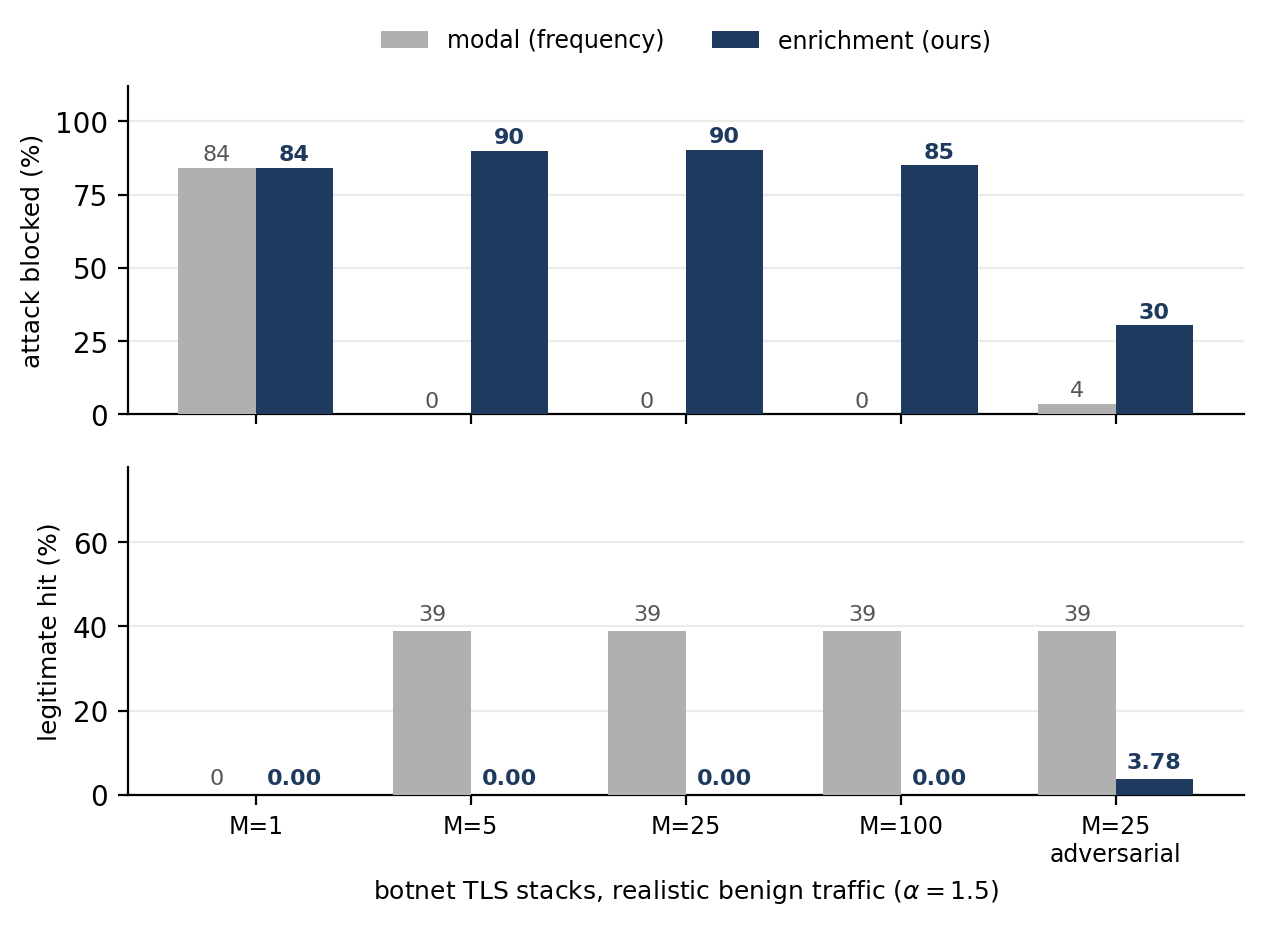
\includegraphics[width=0.76\columnwidth]{figures/fig3_collateral.png}
\caption{Choosing the discriminator by frequency versus by enrichment, under
realistic benign fingerprint concentration ($\alpha = 1.5$). The modal rule holds
only for a monolithic botnet; from five stacks on it blocks no attacker and
$39\%$ of legitimate users. Enrichment is invariant to fragmentation, and under
adversarial fingerprint adoption it declines rather than harms. $n = 15$ seeds.}
\label{fig:collateral}
\end{figure}

Mitigation is only meaningful as a pair: what the derived scope blocks, and what
it costs. We report both over $n = 15$ campaigns per configuration, comparing the
frequency rule against the enrichment rule of Section~\ref{sec:evidence}
(Fig.~\ref{fig:collateral}).

For a monolithic botnet the two agree: $84.0\%$ of attacker sessions blocked at
$0.00\%$ collateral, against $100\%$ for a global endpoint rate limit, which by
definition disconnects every legitimate user of the attacked service. That is the
regime in which the frequency rule was validated, and it is not representative.
From five stacks on, the modal fingerprint of the cluster becomes a
\emph{legitimate} one and the rule inverts: $0.0\%$ of the attack blocked and
$39.0\%$ of legitimate traffic hit. That is worse than doing nothing, since it
imposes the cost of mitigation and delivers none of the benefit. A more concentrated
benign population ($\alpha = 2.0$) raises that collateral to $61.1\%$.

Enrichment removes the failure, blocking $90.0\%$, $90.3\%$ and $85.0\%$ of the
attack at $M = 5$, $25$ and $100$ stacks, in every case at $\mathbf{0.00\%}$
collateral, and reproducing the frequency rule where the latter worked. The
surviving $10$--$15\%$ is the tail of attackers with one-off fingerprints:
scoped mitigation trades completeness for precision.

\textbf{Two conditions bound the result.} The first is adversarial: when the
botnet adopts common benign fingerprints, little is enriched and the rule blocks
$30.4\%$ of the attack at $3.78\%$ collateral, against $3.6\%$ and $39.0\%$ for the
frequency rule. The surgical advantage is largely lost, but it is lost
\emph{safely}: with a stricter $\rho$ the scope declines to name a fingerprint and
degenerates to the global control, the correct report when no discriminator
exists. The
second is the background profile. Moderate drift is tolerable ($\alpha = 2.0$
profile against an $\alpha = 1.5$ episode: $90.3\%$ coverage, $0.45\%$ collateral);
a flat or missing profile is not, since every fingerprint then looks rare, the
benign head scores as enriched, and collateral jumps to $81.2\%$. Coverage is
unaffected throughout, since profile quality governs precision rather than recall,
so maintaining it is a deployment requirement and not an optimisation.

\subsection{Cost and the Choice of $W$}
\label{sec:latency}

Appendix~\ref{app:cost} measures both layers of the pipeline against window
occupancy. Two results carry: admission costs a constant $14$--$19$~ns per
candidate pair, sustaining some $84\,000$ session admissions per second on one
core at $|S_W| = 1\,000$; and detection is flat over a $30\times$ range of $W$
while cluster occupancy, and with it the quadratic pair term that $\Omega(S)$
implies, grows $6.6\times$. Keep $W$ as small as the traffic allows.

\subsection{Statistical Significance}

Paired Wilcoxon tests over the $n = 30$ runs, with Bonferroni correction and
Cohen's $d$. In the distributed regime ($K = 1000$), \textbf{(d)$-$(c)} is
significant at $p_{\mathrm{Bonf}} = 7.5\times 10^{-9}$ with $d = 13.5$, and
\textbf{(d)$-$(a)} at $p_{\mathrm{Bonf}} = 7.5\times 10^{-9}$ with $d = 22.4$.
Effect sizes of this magnitude reflect the controlled nature of synthetic
traffic, which gives near-perfect separation, and should not be read as an
expectation of field performance.

%% ====================================================================
\section{Discussion and Limitations}
\label{sec:discussion}

Five limitations bound the claim; further ones are listed in
Appendix~\ref{app:limitations}.

\textbf{The gain is regime-specific.} Against single-source high-volume attacks,
per-IP or per-session thresholds perform comparably, and on the conventional
real attacks available in public datasets a strong per-session classifier
already reaches $\mathrm{AUC} \geq 0.98$, leaving cross-session reasoning a
marginal margin. The advantage is decisive only when the campaign is distributed
\emph{and} stealthy. This work does not replace volumetric defences; it
complements them. Validating the approach on \emph{captured} stealthy
distributed traffic, which no public benchmark provides, is the single most
important experimental direction.

\textbf{The synthetic evaluation demonstrates a mechanism, not field
performance.} In the synthetic setting the coordination signals present in the
campaign are exactly those measured by configuration (d), and attacker sessions
draw their per-session attributes from real benign distributions. The
per-session non-separability in Table~\ref{tab:ablation} is therefore not an
artefact of a weakened baseline, since four model families with all flow
attributes stay at chance. The mimicry is imposed by construction, so the result
shows the mechanism under an assumption of perfect per-session mimicry rather
than proving performance on a real capture of that regime.

\textbf{Detection and scoping both depend on an observable high-weight
discriminator.} A robustness sweep ($n = 10$) makes the dependency explicit: as
the fraction of origins sharing the TLS fingerprint falls, $\mathrm{AUC}$(d)
decreases monotonically from $1.00$ to $\approx 0.74$ under full randomisation.
That residual above chance is an artefact of a finite benign JA4 pool, so under
internet-scale diversity it should tend to chance. Endpoint convergence does
\emph{not} compensate for the loss of JA4 when legitimate users share the
endpoint, because they converge on it too. Adversaries can forge JA4 with tools
such as \texttt{curl-impersonate}, jitter timing and rotate identities; the
weighted family tolerates partial breakage, since surviving high-weight signals
carry the cluster, but breaking three or more at once degrades it towards chance.
Widespread adoption of Encrypted Client Hello~\cite{ietf2024ech} could likewise
make JA4 unobservable, requiring alternative TLS metadata to compensate.

\textbf{Operational placement.} The framework closes a management loop rather
than emitting labels: detection, evidence and scope come from one pass over the
same graph, so what reaches the operator or a SOAR playbook is a STIX
\emph{course-of-action} already parameterised by the discriminator that justified
the verdict. The sliding window is what makes that affordable
(Section~\ref{sec:latency}). It is a session-plane complement to volumetric
defences at the edge, not a replacement.

\textbf{Parallelism and partitioning.} The rule itself dictates the natural
shard key. Condition (ii) requires every session of $S$ to target the same
endpoint $e$, so partitioning the active window by endpoint evaluates
\texttt{CoordinatedHTTPFlood} \emph{exactly}, with no cross-shard traffic: the
detector becomes embarrassingly parallel over endpoints, and because the window
bounds $|S_W|$, per-shard state does not grow with cumulative traffic volume.
The cost is not zero, though. Sharding by endpoint hides a campaign that spreads
one JA4 across many endpoints, since no shard accumulates enough coordinated
pairs to clear $\tau_{\mathrm{cluster}}$; sharding by JA4 instead preserves those
campaigns and breaks the endpoint condition. No single key preserves all six
sub-relations, and that is a property of $\Omega(S)$ rather than of any
implementation. The design it suggests, unimplemented, is two tiered:
endpoint-sharded workers plus a global sketch over high-weight identifiers to
recover cross-endpoint campaigns; quantifying the recall lost by the first tier
and recovered by the second is a precondition for CDN-scale deployment. Taken together with Section~\ref{sec:latency}, the three
measurements compose one scalability argument: endpoint sharding is exact and
needs no coordination, a small $W$ costs no detection while cutting the
quadratic pair term, and admission is microseconds. In a correctly configured
deployment the quadratic term therefore never binds.

\textbf{The ablation measures representation, not formalism.} Configuration (d)
reaches the graph's evidence through features rather than through SPARQL: a
linear model over the same three cross-session features still attains $0.799$
against $0.495$ for the per-session set, so the AUC gain in
Table~\ref{tab:ablation} is attributable to representing cross-session structure,
not to expressing it in OWL. The symbolic layer is evidenced separately, by
Table~\ref{tab:symbolic}, and only in part: it does not beat the learned model
against a monolithic botnet, and its advantage appears once fragmentation or
adversarial fingerprint adoption make the score distribution unusable for a
zero-false-positive threshold. Readers should keep the two claims apart.

\textbf{Attack-family, protocol and dataset coverage.} The ontology and the
evaluation cover the Slow HTTP DoS family over HTTP/1.1; HTTP/2 attacks and
other application protocols need sub-relations we have not modelled. Real-data
validation spans six attacks (Slowloris, Slowhttptest, HULK, GoldenEye,
HTTP-Flood, DoS-Other) across two datasets, but all of them are laboratory
testbed captures, and the head-to-head comparison with KLAGE is necessarily
single-attack, since that is what KLAGE publishes. That comparison also differs
in granularity and protocol, so reproducing KLAGE under our protocol is required
before any superiority claim.

%% ====================================================================
\section{Conclusion}
\label{sec:conclusion}

We modelled the HTTP session as a first-class ontological entity and replaced
flat cross-session relatedness with six typed sub-properties, weighted by the
attacker's cost of breaking each signal. A SPARQL/SWRL rule fires on their
weighted mass, so that one derivation serves at once as the verdict, the evidence
chain and the scope of the mitigation.

Against stealthy distributed campaigns, per-session detection sits at chance
across four model families given the full flow-feature set, while the framework
detects consistently ($0.50$ vs.\ $0.98$ ROC AUC; $d = 13.5$); on conventional
real attacks the gain is marginal, because a strong per-session classifier already
suffices. On the mitigation side the study produced a negative result worth as
much as the positive one: scoping by the property the cluster mostly shares
selects a legitimate fingerprint once the botnet spans more than one TLS stack,
blocking users instead of attackers. Enrichment over a profile of normal traffic
restores $85$--$90\%$ coverage at $0.00\%$ collateral. And measured as a detector,
that symbolic path recovers $90\%$ of a 25-stack campaign where the learned model
recovers $36\%$ at the same zero-false-positive operating point. That gap is
hidden by the AUC, and it is our clearest evidence that the graph earns its
place. Immediate
directions are HTTP/2 attacks and a captured stealthy campaign, which no
benchmark yet provides.

\section*{Acknowledgment}
We thank Azion Technologies for authorising the aggregate fingerprint measurement
of Section~\ref{sec:method}.

\bibliographystyle{IEEEtran}
\bibliography{references}

%% ====================================================================
\appendices

\section{Instantiation of the \texttt{relatedBy} Sub-Relations}
\label{app:algorithms}

For each pair $(s_a,s_b)$ of sessions active in $W$, the following decision
procedures determine whether the corresponding edge is instantiated.

\textbf{\texttt{TLSFingerprint}.} Two-stage match: exact equality of the full
JA4, or --- failing that --- near variants (same transport/TLS-version/ALPN
prefix, at most one symbol of difference in the ordered cipher or extension
blocks), instantiated with a \emph{ja4\_distance = 1} annotation. This absorbs
version drift within one client library without admitting spurious matches
across distinct stacks. Cost $O(1)$ per pair.

\textbf{\texttt{ReusedIdentity}.} Instantiated on any non-empty overlap between
the observed identity sets, $(\mathrm{cookie}(s_a) \cap \mathrm{cookie}(s_b))
\cup (\mathrm{token}(s_a) \cap \mathrm{token}(s_b)) \cup (\mathrm{user}(s_a) \cap
\mathrm{user}(s_b)) \neq \emptyset$. JWTs are decoded and compared by the
\texttt{sub} claim; cookies and usernames are normalised (trim, lower-case).
Cost $O(1)$ amortised with an inverted index.

\textbf{\texttt{TemporalPattern}.} With $\Delta(s)$ the sequence of
inter-arrival times, we compute
$d_{\mathrm{DTW}}(s_a,s_b) = \mathrm{DTW}(\Delta(s_a),\Delta(s_b)) /
\max(|\Delta(s_a)|,|\Delta(s_b)|)$ and instantiate when
$d_{\mathrm{DTW}} \leq \tau_{\mathrm{DTW}}$. Sessions with fewer than three
requests are skipped. FastDTW under a constant-width Sakoe--Chiba band reduces
the per-pair cost from $O(n^2)$ to $O(n)$, and locality-sensitive hashing over
summary vectors ($\bar\delta$, $\sigma_\delta$, $\delta_{\min}$,
$\delta_{\max}$, entropy) avoids all-pairs comparison.

\textbf{\texttt{PayloadSignature}.} With
$\mathbf{p}(s) = (\overline{\mathrm{len}}, \sigma_{\mathrm{len}}, h_{\mathrm{UA}},
h_{\mathrm{CT}})$ --- mean and standard deviation of body size, plus hashes of
the dominant User-Agent and Content-Type --- the edge is instantiated when
cosine similarity exceeds $\tau_{\mathrm{payload}}$. Cost $O(1)$ given
precomputed vectors.

\textbf{\texttt{EndpointConvergence}.} Instantiated when both sessions converge
on the same endpoint, under path-pattern normalisation
(\texttt{/api/users/12345} $\rightarrow$ \texttt{/api/users/\{id\}}) by default;
an additional exact-path match annotates the edge with \emph{exact = true}. Cost
$O(1)$ with a prefix-tree index.

\textbf{\texttt{NetworkProximity}.} Instantiated on a shared IPv4 /24 (or IPv6
/48) prefix, or a shared ASN, or both; when both hold the edge is annotated
\emph{strong = true}. ASN resolution uses current BGP tables. Cost $O(1)$ with
an inverted prefix index.

\begin{figure}[t]
\footnotesize
\hrule\vspace{2pt}
\begin{verbatim}
# SWRL (Horn): instantiate one sub-relation
ApplicationSession(?a) ^ ApplicationSession(?b) ^
  differentFrom(?a,?b) ^
  tlsJa4(?a,?j) ^ tlsJa4(?b,?j)
  -> relatedByTLSFingerprint(?a,?b)

# SPARQL: weighted aggregation over the cluster
SELECT ?e (SUM(?w) AS ?omega) (COUNT(*) AS ?pairs)
WHERE { ?a kg:targets ?e . ?b kg:targets ?e .
        ?a ?rel ?b .
        ?rel rdfs:subPropertyOf kg:relatedTo ;
             kg:coordinationWeight ?w .
        FILTER(STR(?a) < STR(?b)) }
GROUP BY ?e HAVING (SUM(?w) >= ?tau)
\end{verbatim}
\vspace{-4pt}\hrule
\caption{Verdict as derivation: Horn rules materialise typed cross-session edges;
a SPARQL aggregation applies the ontology-declared weights and fires the rule.
The bindings that satisfy the query \emph{are} the evidence chain.}
\label{fig:rules}
\end{figure}

\section{Weight Calibration}
\label{app:calibration}

Empirical calibration depends critically on the realism of the traffic. On
laboratory datasets --- a few dozen distinct JA4 fingerprints --- optimisation
even inverts the sign of the TLS signal, because benign sessions share
fingerprints more than partially coordinated campaigns do; this is a testbed
artefact of low JA4 diversity, absent from the real internet.

In the realistic scenario (thousands of legitimate JA4 fingerprints, users
hitting the attacked service), we calibrate by maximising per-session
attack-vs-benign ROC AUC over the score
$w_{\mathrm{tls}}\,z(\mathrm{ja4}) + w_{\mathrm{ep}}\,z(\mathrm{endpoint\ conv.})
+ w_{\mathrm{net}}\,z(\mathrm{net\ prox.})$ with standardised attributes, over
the grid $\{0.3\ldots1.0\}^3$ (125 combinations, 60 scenarios, 91\,500
sessions). The result corroborates the proposed ordering: the best vector is
$(w_{\mathrm{tls}}{=}1.0,\ w_{\mathrm{ep}}{=}0.3,\ w_{\mathrm{net}}{=}0.3)$, and
the TLS fingerprint is the only individually discriminative signal (isolated
$\mathrm{AUC} = 0.93$, against $0.50$ for endpoint convergence and $0.58$ for
network proximity). The weights of Fig.~\ref{fig:ontology}
$(1.0,\ 0.6,\ 0.3)$ attain the same optimal $\mathrm{AUC} = 0.943$ and are
insensitive to $\pm20\%$ perturbation (no measurable drop). Calibration
therefore validates the \emph{ordering}; in the pure same-service regime the
medium and low weights are not separately identifiable, since in isolation both
sit near chance, and their absolute values remain open pending production
traffic with partial and conflicting signals.

\section{Additional Limitations}
\label{app:limitations}

\textbf{Session and identity instrumentation.} The approach assumes sessions,
identities and TLS fingerprints can be extracted from traffic events; where that
instrumentation is partial or noisy, performance degrades.

\textbf{Graph maintenance cost.} The symbolic figures of
Section~\ref{sec:latency} come from an in-memory \texttt{rdflib} reference
implementation rather than the Jena/TDB2 backend, so they are an upper bound,
and scaling to CDN-scale traffic requires the horizontal partitioning discussed
in Section~\ref{sec:discussion}, which we did not implement.

\textbf{Protocol coverage.} The current ontology covers the Slowloris family and
direct descendants over HTTP/1.1. HTTP/2 attacks and other application
protocols (DNS, gRPC) need additional sub-relations.

\textbf{Dataset breadth.} Real-data validation covers one dataset and one attack
for the head-to-head comparison, plus six attacks across CICIDS2017 and
CIC-IoT2023 for the regime analysis. RT-IoT2022, CIC-DDoS2019 and anonymised
production traffic remain future work.

\textbf{Explanation validation.} Evidence chains were assessed for structural
completeness and actionability ($7/7$), but \emph{perceived} actionability --- a
human-analyst study of time-to-decision and comprehension --- was not conducted.

\begin{figure}[h]
\centering
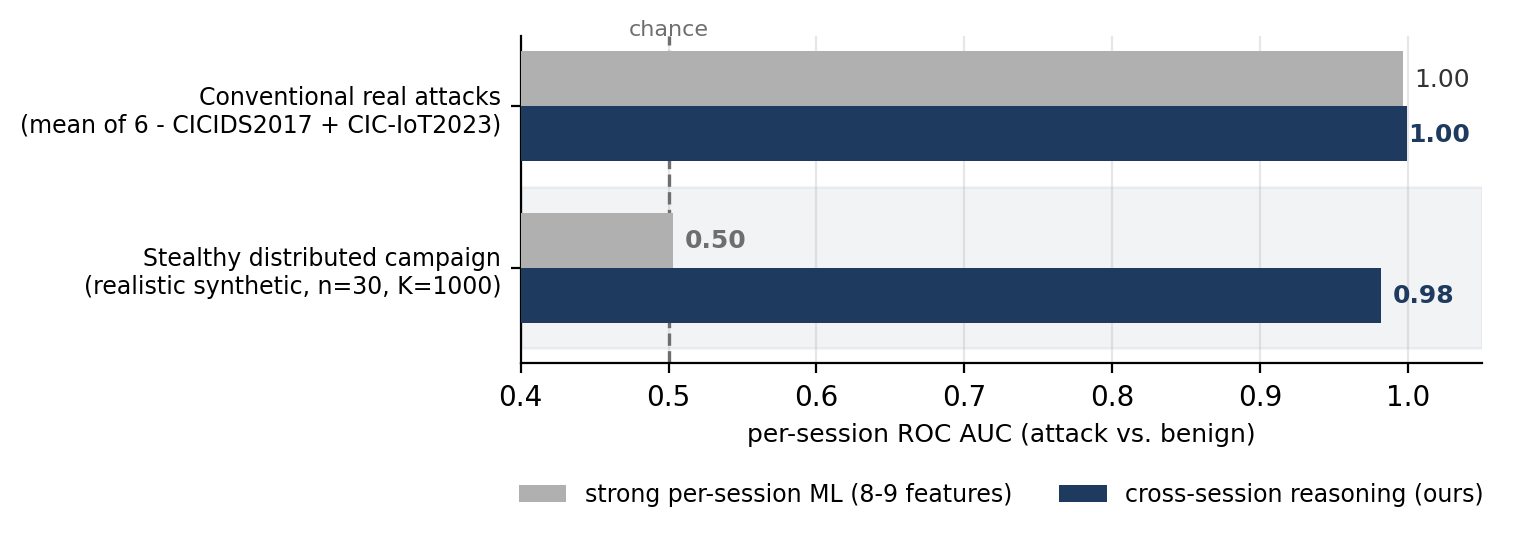
\includegraphics[width=\columnwidth]{figures/fig2_regime.png}
\caption{Where cross-session reasoning is \emph{needed}. On conventional real
attacks a strong per-session classifier already saturates; only in the stealthy
distributed regime does per-session detection collapse to chance while
cross-session reasoning holds.}
\label{fig:regime}
\end{figure}

\section{Cost Model and Window Sensitivity}
\label{app:cost}

\begin{figure}[h]
\centering
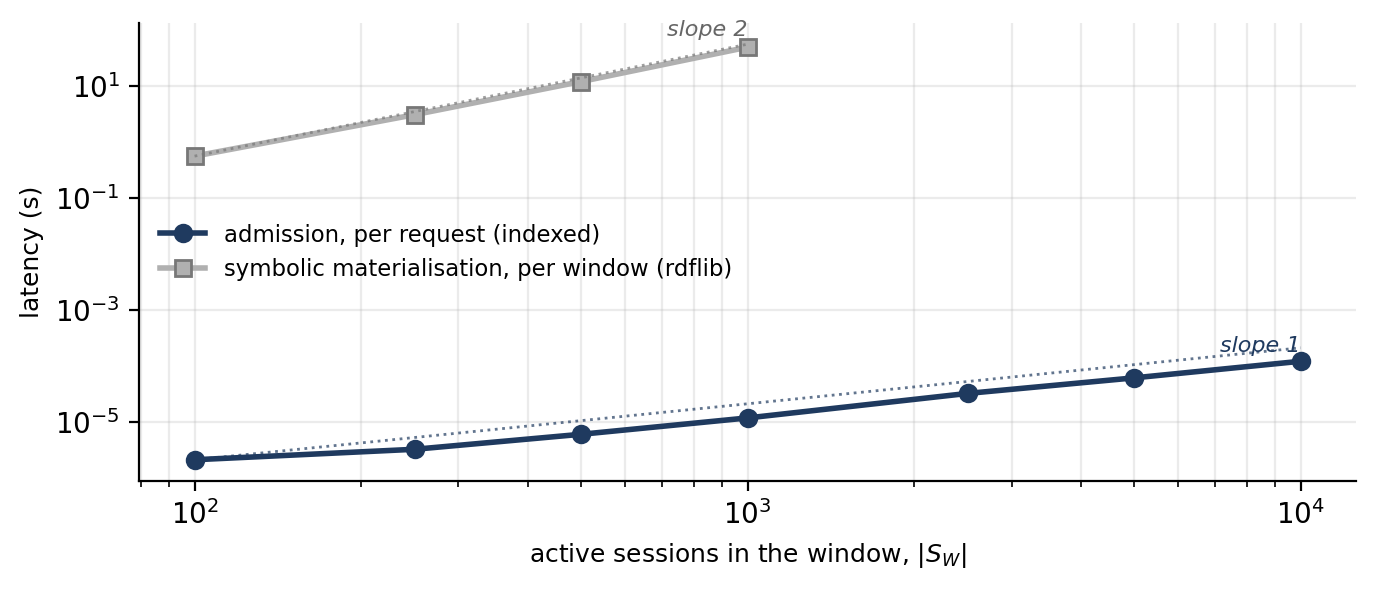
\includegraphics[width=\columnwidth]{figures/fig4_latency.png}
\caption{Cost of the two layers against window occupancy. Per-request admission
is linear in $|S_W|$ and stays in the microsecond range; per-window symbolic
materialisation is linear in the number of RDF edges, which is itself quadratic
in $|S_W|$. Reference slopes anchored on the first point of each series.}
\label{fig:latency}
\end{figure}

The two layers run at different rates --- admission happens per request,
symbolic materialisation and the $\Omega$ aggregation per window --- so we time
them separately, on a synthetic window in the realistic same-service mix (30\% of
sessions in one campaign sharing a botnet JA4, benign JA4 from a pool of 2\,000,
eight endpoints, dispersed /24s); medians over three repeats on one core. This
is a cost model of the algorithm as specified, not a system benchmark: the
admission path is a direct implementation of the inverted-index scheme of
Section~\ref{sec:pipeline}, and the symbolic layer runs on an in-memory
\texttt{rdflib} reference implementation rather than the Jena/TDB2 backend used
for the dataset pipeline, so its figures are an upper bound.

Admission behaves as the bound predicts (Fig.~\ref{fig:latency}): median latency
grows from $2.1\,\mu$s at $|S_W| = 100$ to $122\,\mu$s at $|S_W| = 10\,000$,
tracking the candidate-pair count (148 to 6\,495 edges per admission) at a
constant $14$--$19$~ns per pair.

The symbolic layer is orders of magnitude more expensive: $0.56$~s at
$|S_W| = 100$ rising to $49.7$~s at $|S_W| = 1\,000$. Read per unit of work,
however, cost stays constant at $\approx 187\,\mu$s per materialised RDF edge
across all sizes, so the layer is \emph{linear in edges}; it is the edge count
that grows quadratically, because $\Omega(S)$ is defined over pairs. The
quadratic term is thus a property of the rule rather than of the backend, and it
points at the deployment split the architecture already implies: detect on the
indexed admission path, and materialise RDF only for the clusters that fire ---
the evidence-chain subset, not the whole window.

\begin{table}[h]
\centering
\caption{Window sweep, $K = 1000$, $n = 10$ seeds. Detection is flat across a
$30\times$ range of $W$ while cluster occupancy --- and hence the quadratic pair
term --- grows with it.}
\label{tab:window}
\footnotesize
\setlength{\tabcolsep}{4pt}
\begin{tabular}{@{}rrrcccc@{}}
\toprule
$W$ (s) & clusters & mean $|S|$ & (a) & (b) & (c) & (d) \\
\midrule
   60 & 16 & 132 & 0.505 & 0.508 & 0.664 & 0.976 \\
  120 & 11 & 207 & 0.505 & 0.508 & 0.663 & 0.977 \\
  300 &  6 & 364 & 0.505 & 0.508 & 0.664 & 0.977 \\
  600 &  4 & 557 & 0.505 & 0.508 & 0.664 & 0.978 \\
 1800 &  3 & 867 & 0.505 & 0.508 & 0.664 & 0.978 \\
\bottomrule
\end{tabular}
\end{table}

Appendix~\ref{app:cost} measures the two layers of the pipeline --- per-request
admission and per-window symbolic materialisation --- against window occupancy.
Two consequences belong here. The per-request path is not the bottleneck:
admission costs a constant $14$--$19$~ns per candidate pair, so median latency
stays in the microsecond range and grows linearly in $|S_W|$, sustaining roughly
$84\,000$ session admissions per second on one core at $|S_W| = 1\,000$. And that
cost profile settles how to pick $W$: over a $30\times$ range detection does not
move --- (d) goes from $0.976$ to $0.978$ between $60$~s and $1800$~s, (a) and (c)
not at all --- while mean cluster occupancy grows $6.6\times$, and with it the
quadratic pair term that $\Omega(S)$ implies. The invariance follows from the
discriminative feature being a share, which is scale-free. Keep $W$ as small as
the traffic allows: a larger window buys no detection and costs roughly its
square.

$W$ enters only through detection-cluster assignment, so the sweep recomputes
the cross-session features on the same cached scenarios. Table~\ref{tab:window}
shows detection is insensitive to it over $60$--$1800$~s: the discriminative
feature is the fraction of a cluster sharing one JA4, a ratio that does not
change as the cluster grows, whereas cluster size alone carries little --- which
is why (c) sits at $0.664$ throughout. Two bounds on this result: the scenarios
target a single endpoint, so $W$ is the only clustering knob and a multi-endpoint
deployment with interleaved campaigns may behave differently; and $W$ must still
be long enough for a cluster to form at all, which at $W = 60$~s already means
$\approx 132$ sessions here.

\begin{figure}[t]
\footnotesize
\hrule\vspace{2pt}
\begin{verbatim}
"@type": "kg:CoordinatedHTTPFlood",
"kg:clusterSize": 6, "kg:coordinationScore": 10.8,
"kg:activatedSubRelations": [
 {"@type": "kg:relatedByEndpointConvergence",
  "kg:coordinationWeight": 0.6, "kg:linkedPairs": 15,
  "kg:weightedContribution": 9.0},
 {"@type": "kg:relatedByNetworkProximity",
  "kg:coordinationWeight": 0.3, "kg:linkedPairs": 6,
  "kg:weightedContribution": 1.8}],
"kg:derivedMitigationScope": {
  "kg:endpoint": "192.168.10.50:80",
  "kg:srcNet24":  "172.16.0.0/24"}
\end{verbatim}
\vspace{-4pt}\hrule
\caption{Evidence chain emitted for the CICIDS2017 DoS-Other cluster (JSON-LD,
abridged). Every term of $\Omega(S) = 10.8$ is attributable to a sub-relation,
a pair count and a weight, and the last field is the filter actually applied.
The STIX~2.1 export carries the same content as an \emph{indicator} pattern
plus a \emph{course-of-action} linked by \emph{mitigates}.}
\label{fig:chain}
\end{figure}

\section{Reproducibility}
\label{app:repro}

The reference implementation is available at
\url{https://github.com/Natanael0liveira/knowledge-graph-ddos-article} under a
permissive licence, organised by experimental stage: the extraction pipeline
(PCAP $\rightarrow$ JA4 and flows $\rightarrow$ sessions $\rightarrow$ graph);
the calibrated synthetic generator, including the three realism parameters of
Section~\ref{sec:method} --- Zipf exponent of benign fingerprint popularity,
number of botnet TLS stacks, and adversarial adoption of common benign
fingerprints --- with the canonical and adversarial scenario configurations; the
ablation, the academic baselines and the four model families; the statistical
runner; the comparison against published state of the art; the symbolic layer
(SWRL rules plus the SPARQL aggregation, with weights read from the ontology);
and the evidence and mitigation modules.

Both scope derivations ship side by side, deliberately: the frequency rule that
fails and the enrichment rule that replaces it, so that the negative result of
Section~\ref{sec:collateral} is reproducible and not merely asserted. The
background profile the enrichment test needs is produced by an attack-free
generator run, so no labels enter the decision path at any point. The cost model
of Appendix~\ref{app:cost} requires no dataset and runs anywhere.

Seeds are fixed, orchestration is driven by Makefiles, and artefacts --- figures,
calibrated distributions and aggregated results --- are versioned; every table
and figure in this paper regenerates from a single command per stage. The OWL
ontology is provided in RDF/XML, with every \texttt{relatedBy} sub-property
annotated with its \texttt{coordinationWeight}. We intend to submit these
artefacts to the Artifact Evaluation track.

\end{document}
